\documentclass[letterpaper,twocolumn,amsmath,amssymb,pre,aps,10pt]{revtex4-1}
\usepackage{graphicx} % Include figure files
\usepackage{color}
\usepackage{nicefrac} % Include for inline fractions

\newcommand{\red}[1]{{\bf \color{red} #1}}
\newcommand{\green}[1]{{\bf \color{green} #1}}
\newcommand{\blue}[1]{{\bf \color{blue} #1}}
\newcommand{\cyan}[1]{{\bf \color{cyan} #1}}

\newcommand{\davidsays}[1]{{\color{red} [\green{David:} \emph{#1}]}}
\newcommand{\jpsays}[1]{{\color{red} [\blue{Jordan:} \emph{#1}]}}
\newcommand{\tssays}[1]{{\color{red} [\cyan{Tanner:} \emph{#1}]}}

\begin{document}
\title{Dynamic Stochastic Approximation Monte Carlo}

\author{Jordan K. Pommerenck} \author{Tanner T. Simpson}
\author{Michael A. Perlin} \author{David Roundy}
\affiliation{Department of Physics, Oregon State University,
  Corvallis, OR 97331}

\begin{abstract}
  We present several histogram methods and compare the performance and
  efficiency at treating the square-well fluid.
\end{abstract}

\maketitle

\begin{figure}
  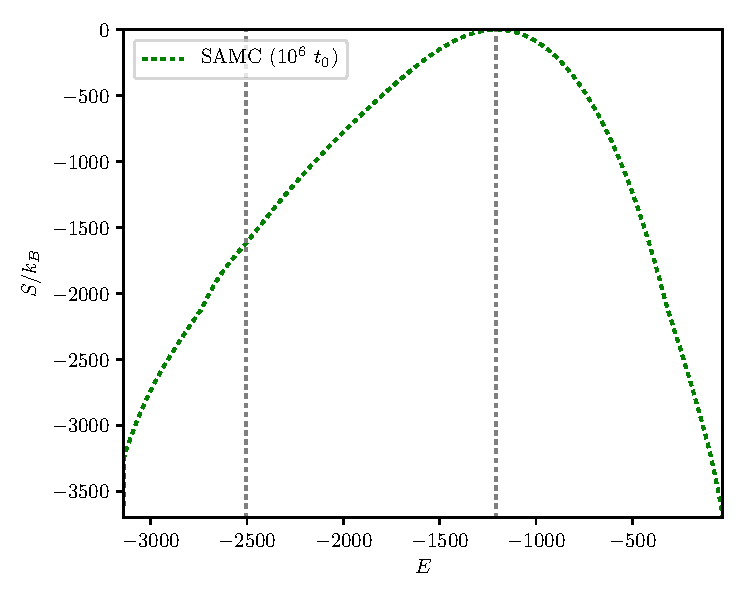
\includegraphics[width=\columnwidth]{figs/N500-lndos-comparison}
  \caption{Put this in the right place}
\end{figure}

\section{Introduction}
Over the past several decades a number of broad histogram Monte-Carlo
simulation algorithms have been developed which calculate the
thermodynamic properties of various systems for all temperatures.  The
development began with the original histogram method, which used a
single canonical Monte Carlo simulation to predict properties for
nearby temperatures~\cite{ferrenberg1988new}.  For large simulations
this approach is limited to a narrow temperature range because a single
canonical simulation explores only a small range of energies.  This led
to a variety of ``broad'' (or ``flat'') histogram
methods~\cite{penna1996broad, penna1998broad, swendsen1999transition,
wang2001determining, wang2001efficient, trebst2004optimizing}, which
attempt to explore a wide range of energies.  These methods also
benefit in that they are unlikely to be trapped in a low enetropy state.

Wang and Landau introduced an algorithm that uses an update factor and
a statistical histogram to compute the density of states of a given
system~\cite{wang2001determining, wang2001efficient}.  While the method
is incredibly powerful, it has several user-defined parameters.  This
can make its application to a variety of systems something of an
art-form since the user needs to determine the ideal parameters for the
particular system being studied.  Also, detailed balance is violated
(although only for short periods of time), ensuring that convergence is
not guaranteed.  This raises several questions such as when the method
does converge, what rate will the method converge to the correct
density of states. Also, how can the user appropriately decide what
parameters to choose so that the algorithm solves the problem in the
most ideal way.

Transition Matrix Monte Carlo~\cite{wang1999transition,
swendsen1999transition, fitzgerald2000monte} became an attractive
complimentary simulation algorithm to Wang-Landau, in that, if detailed
balance is ensured, the system is guaranteed to converge.  Unfortunately,
the algorithm can be considerably more difficult to implement when
compared to Wang-Landau: in particular, due to the infinite temperature
transition matrix~\cite{wang2002transition}.  Also, the time necessary
for the density of states to converge could be considerable
due to the algorithm spending too much time exploring low energy states.
Unlike WL, TMMC does not require a prior knowledge of the energy range of
the system.

Shell et al.~\cite{shell2003improved, shell2004flat} originially
implemented Wang-Landau Transition Matrix Monte Carlo (WL-TMMC) in an
effort to quickly explore the energies of a given system using WL then
switch over to TMMC to guarantee convergence. Considerable effort has
been spent trying to determine the flatness criteria and cutoff for the
WL portion, but there remains no rigorous systematic way to determine
these parameters~\cite{rane2013monte}.  The algorithm is first run for
several trial simulations and/or `experience' is used to determine the
best parameters for a users particular system of
study~\cite{siderius2013use}.

Around the same time, the convergence rate for WL was being
explored~\cite{zhou2005understanding,lee2006convergence,
belardinelli2007wang}. It was found that utilizing modification factors
that decrease faster than $1/t^2$ leads to
nonconvergence~\cite{belardinelli2007fast}.  This leads to the so-called
$1/t$-WL algorithm which ensures that excess CPU time is not wasted by
continuing to perform calculations once the error in the density of
states becomes saturated~\cite{belardinelli2008analysis}. An effort to
reduce the number of user defined parameters of WL and formulate a
theory for why the method converges despite detailed balance being
violated although infrequently was also being undertaken.

Liang, Liu, and Carrol began to consider whether WL could be considered
a special case of Stochastic Approximation whose convergence could be
mathematically proven~\cite{liang2006theory, liang2007stochastic}. In
2007, Liang et al.~\cite{liang2007stochastic} argued that WL can be
considered a form of Stochastic Approximation Monte Carlo (SAMC). While
SAMC can guarantee convergence, the method still has a system specific
user-defined variable which makes applying this algorithm to arbitrary
systems difficult.

In this work, we have developed a novel algorithm based on SAMC that
does not require user-defined inputs and therefore should be easily
applicable to a given system.  We call this method SAD (Dynamic
Stochastic Approximation), and will discuss it in detail in the methods
section. We compare it along with several broad histogram methods
which include TMMC, WL, WL-TMMC, and SAMC.

We consider the square-well fluid i.e. a system of particles whose
interactions are governed by a square-well
potential~\cite{singh2003surface, barker2004perturbationSW}.  The
square-well potential is an ideal test-bed as it is the simplest model
that ensures both attractive and repulsive forces are experienced by
interacting particles~\cite{barker1967-SW-perturbation, vega1992phase}.
The potential $U(\textbf{r})$ for such a system is given by
\begin{equation}
 U(\textbf{r})=\begin{cases} \infty &
 \lvert\textbf{r}\rvert< \sigma\\-\epsilon &
 \sigma<\lvert\textbf{r}\rvert<\lambda\sigma\\0 &
 \lvert\textbf{r}\rvert > \lambda\sigma\end{cases}
\end{equation}
where $\sigma$ is the hard-sphere diameter of the particle, $\lambda$ is the
reduced range of the potential well, and $\epsilon$ is its depth.

The organization of this paper is as follows: In Section II, we
describe in detail several broad-histogram methods used to calculate
the density of states for the liquid-vapor system.  Section III
contains the results and comparison of the methods applied to the
square-well fluid.  In Section IV, we discuss the performance of the
various methods applied to the model system.

\section{Methods}

In this work, We compare a variety of broad histogram methods.  We
outline the general workings of each algorithm that we developed in
detail while summarizing algorithms that originated elsewhere.  The
following methods are introduced and applied to the square-well fluid:
Transition Matrix Monte-Carlo (TMMC), Wang-Landau (WL), Wang-Landau
Transition Matrix Monte-Carlo (WL-TMMC), Stochastic Approximation
Monte-Carlo (SAMC), and Dynamic Stochastic Approximation
(SAD).

\subsection{TMMC Algorithm}
The Transition Matrix Monte-Carlo (TMMC) method as introduced by
Fitzgerald et al. consists of three primary steps.  The first two steps
are common to the Metropolis algorithm while the third makes use of the
actual transition probabilities~\cite{fitzgerald2000monte}.

\subsubsection{define a transition probability}
Assuming that the system under study is in a state denoted old, and a
proposed transition is made to a new state denoted new, the probability
is defined as
\begin{align}
  p_{old \rightarrow new} = p_{new \rightarrow old}
\end{align}
where we have allowed the probabilies to be equal for simplicity of
presentation.

\subsubsection{define an acceptance probability}
The probability for accepting a transition from an old state to a new
one can be defined
\begin{align}
  p_{a} = \min\bigg[1,\frac{\alpha_{new\rightarrow old}}
  {\alpha_{old \rightarrow new}}\frac{\pi_{new}}{\pi_{old}}\bigg]
\end{align}
where $\alpha_{new\rightarrow old}$ is the probability of generating a
new system configuration the old.  For conventional Monte-Carlo moves
$\alpha_{old \rightarrow new} =\alpha_{new\rightarrow old}$ although
for advanced Monte-Carlo moves this would not be the
case~\cite{paluch2008comparing, siepmann1990method}.  The probabily of
observing the system in the old state can be found based on the
ensemble constraints placed on the system.  Fitzgerald et al.
considered the system of interest using the canonical ensemble;
however, the extension to other ensembles is quite natural.
\begin{align}
  \pi_{old} = \frac{e^{-\beta E_{old}}}{Z}
\end{align}
\subsubsection{define a bookkeeping step}
The third step in the TMMC algorithm consists of recording the data in
a collection matrix (the unormalized transition histogram matrix).
\begin{align}
  C_{N,\delta} = C_{N,\delta} + p_{a}\\
  C_{N,0} = C_{N,0} +(1 - p_{a})
\end{align} If $\delta=0$, that is, the energy state has not been
changed, then only $C_{N,0}$ is incremented by unity. Fitzgerald et
al.~\cite{fitzgerald2000monte} showed that defining the third step this
way results in a uniform improvement over using histogram estimators to
determine the particle number probability distribution (PNPD).

\subsection{Wang-Landau Algorithm}

The Wang-Landau Algorithm developed by Wang and Landau proposes a
random walk in energy space in order to estimate the density of
states~\cite{wang2001efficient,wang2001determining, landau2014guide}.
Wang-Landau's major tenant is that when counting the histogram
$H(\epsilon)$, the energy occurrences should form a flat distribution.
The criteria for flat sampling is given by
\begin{equation}
	\frac{\min_{\epsilon} H(\epsilon)}
	{\big\langle H(\epsilon)\big\rangle }
	> \eta
\end{equation}
where $\eta$ is usually set to $0.80$ and determines how many times
each energy is sampled relative to the mean number of visits.
Difficulties can occur with this flatness criteria due to the fact that
some energies on a given energy range might never be
sampled~\cite{haber2014transition}. The algorithm is briefly outlined
below where $w$ represents the weights:
\begin{equation}
	\ln{D_{i+1}(\epsilon,N)}=\ln{D_{i}(\epsilon,N)}
	+\gamma
\end{equation}
\begin{equation}
	\gamma_{i+1}=\frac{u}{2} \gamma_{i}
\end{equation}
for $u$ typically greater than 1 and $\gamma$ is the modification
factor for the density of states.  A new configuration for the density
of states with a probability given by the following is chosen:
\begin{equation}
	\mathcal{P}(\epsilon_\text{old} \rightarrow \epsilon_\text{new})
	= \min[1,e^{\ln{D(\epsilon_\text{old})}-\ln{D(\epsilon_\text{new})}}]
\end{equation}
The entire process is repeated until a desired cutoff is reached.

\subsection{WL-TMMC Algorithm}

Wang-Landau Transition Matrix Monte-Carlo (WL-TMMC) method as proposed
by Shell and coworkers~\cite{shell2003improved,shell2004flat} takes
advantage of the ease of implementation and applicability to a variety
of systems, while making use of a transition matrix to address WL
weaknesses, such as its limited statistical accuracy plateau.
This WL version is more accurate for a given number of simulation steps.

\paragraph{Initializing Wang-Landau:} We begin the simulation by
defining a minimum important energy and a maximum entropy state. In
traditional Wang-Landau the WL factor begins at 1.0 and the factor is
modified by 2.0 until the simulation is cutoff typically around
$10^{-10}$.  Rane et. al. published an implemenation of
WL-TMMC~\cite{rane2013monte} that suggested using a WL factor between
1.0 and $10^{-2}$ with a cutoff $<10^{-5}$. In our implementation of
WL-TMMC, we set the WL factor to be 1 and the cutoff to be either
$10^{-4}$ or $10^{-10}$. A single sweep is defined as each macrostate
being sampled a number of times in this case 10,000 (although 100 is
often sufficient for small systems). Wang-Landau sets a flatness
criteria~\cite{wang2001determining, wang2001efficient,
hatch2015computational, mahynski2017predicting} for the accumulated
histogram usually between 0.75 to 0.90.  In the original
implementation, it was found to be sufficient that each macrostate is
visited at least once (each histogram bin has one
entry)~\cite{shell2003improved}; however, for other systems this is
rarely sufficient.  The goal of this WL initialization is to prefill
the transition matrix for the next portion of the simulation.
\paragraph{Initializing TMMC:} Prefilling the transition
matrix is necessary because if numerous zeros existed in the collection
matrix, the infinite temperature transition matrix would be
ill-defined.  Sampling over large ranges of density of states would
therefore take an unacceptable length of time to
complete~\cite{shell2003improved, shen2014elucidating}.  The transition
matrix in terms of the collection matrix is given as
follows:
\begin{align}
\widetilde{T}_{\infty}(I\rightarrow J) = \frac{C(I,J)}
{\sum_{K} C(I,K)}
\end{align}
We now run the TMMC portion of the simulation.
%Siderius does this for 20 additional sweeps (does about 8 sweeps for
%WL).  We do this until we reach a defined number of iterations. We
%have not yet implemented a biasing function to control acceptance rate
%of trial moves but we could? at some point.
The acceptance probability is written in terms of the infinite temperature
transition matrix.
\begin{align}
  P_{acc}(i\rightarrow j) = \min\bigg[1,\frac{\widetilde{T}_{\infty}(J\rightarrow I)}
  {\widetilde{T}_{\infty}(I\rightarrow J)}\bigg]
\end{align}
This probability is only used to control actual transitions not update
the collection matrices.

\subsection{SAMC Algorithm}
SAMC can be applied as a dynamic importance sampling algorithm that
uses an update factor to explore energy
space~\cite{liang2007stochastic, werlich2015stochastic,
schneider2017convergence}.  The update factor is defined in the
original implementation~\cite{liang2007stochastic} in terms of an
arbitrary tunable parameter $t_0$ and a scale factor $\gamma_0$.
\begin{align}
\gamma_{t}^{\text{SA}} =\gamma_0 \frac{t_0}{\max(t_0,t)}
\end{align}
SAMC offers several advantages over other broad histogram methods
including proven convergence. It has been shown that if
$F_{t}^{\text{SA}}$ satisfies two conditions the estimator is proven to
converge to the real DOS~\cite{liang2006theory, liang2007stochastic}.
\begin{align}
\sum_{t=1}^\infty \gamma_{t}^{\text{SA}} = \infty \quad\textrm{and}\quad
\sum_{t=1}^\infty (\gamma_{t}^{\text{SA}})^\zeta < \infty
\end{align}
where $\zeta \in \{1,2\}$.  Unlike WL and WL-TMMC, the energy range need
not be known a priori.  The time to converge depends only on the choice of
parameters $t_0$ and $\gamma_0$.
Unfortunately, only by performing many computational runs might the user
determine what SAMC arbitrary parameters to choose.  This has lead us
to develop a systematic way (which we will discuss in the next section)
for the simulation to determine what $t_0$ should be.

\section{SAD Algorithm}
\subsubsection{The theory behind SAD}
The SAD (Dynamic Stochastic Approximation) method is a version of the SAMC
Algorithm that attempts to dynamically choose the modification factor
rather than relying on system dependent parameters such as $t_0$ or
$\gamma_0$.  There is an immediate advantage of such an algorithm where
parameters are chosen independent of system size or type. Each
Broad-Histogram method has unique advantages and disadvantages.
Wang-Landau requires an energy range for initialization.  SAMC removes
this energy range requirement but requires simulating every possible
energy. Our proposed method SAD requires the user to input
$T_\text{min}$ which is an immediate disadvantage of the method;
however, this allows the user to define an energy simulation
range between $T_\text{min}$ and $\infty$. Setting a physical parameter
such as a minimum temperature $T_\text{min}$ is intuitive vs. a user
needing to know a prior either an energy range or some unphysical
parameter $t_0$.

While for SAMC the update factor is defined in the original
implementation, for SAD the update factor $\gamma_{t}^{\text{SA}}$ can
be thought of as $\nicefrac{\text{d}S}{\text{d}t}$. This tells us that
$t_0$ should have dimensions of entropy.  We argue that we can write
this entropy `term' geometrically as an area bounded by the $\ln{D(E)}$
i.e. the entropy. This gives the following
\begin{align}
\gamma_{t}^{\text{SA}} =
\frac{N_E}{t}\frac{E_{\text{max}}-E_{\text{min}}}{3T_{\text{min}}}
\end{align}
where $N_E$ is the number of energies that have been found. The change
in the entropy the minimum temperature can be thought of as a slope of
the triangle made by connecting the minimum important energy and the
maximum entropy state.  The factor of $3$ comes from the ratio of areas
bounded by the $\ln{D(E)}$ and the minimum temperature line. The update
factor has the same $1/t$ behavior as the original SAMC algorithm;
however now every time a new energy is discovered during the course of
the simulation, the update factor experiences a jump. This behavior
allows SAD to dynamically prevent the update factor from decreasing too
rapidly. In contrast to SAD, Fig.~\ref{fig:gamma-vs-t}. shows the
monotonic decrease of the update factor for SAMC.  The update factor
for WL decreases like a step function while the update factor for SAD
dynamically fluctuates around a value less than 1 for early MC moves
(while finding new energy states).  Ultimately once all energy states
have been found, the update factor for SAD decreases in the same
monotonic fashion as SAMC.

\subsubsection{High and Low energy racheting}
Since SAD explores all energy states it is imperative that the method
have a reasonable idea about where the minimum important energy and
maximum entropy state are located in energy space. Since these are not
user input parameters such as they are for methods like WL-TMMC, the
simulation is responsible for determining and updating these energy
locations. In order to prevent, the method from experiencing errors
near the energy extrema, we employ a high energy $\epsilon_H$ and a low
energy $\epsilon_L$ to define the range over which the energy histogram
is made flat. $\epsilon_H$ is the highest ever value that the maximum
entropy state has taken while $\epsilon_L$ is the lowest ever value
that the minimum important energy has taken. SAD uses these two
energies to control the weights $w(E)$ above $\epsilon_H$ and
$\epsilon_L$. If the energy $E$ is greater than $\epsilon_H$ then the
weights can be calculated as ~\jpsays{equation formatting problems!}
\begin{equation}
\begin{aligned}
\ln w(E) = \max(\ln w(E) + \gamma, \\
    \ln w(\epsilon_H) + \log(\gamma + e^{\ln w(E)-\ln w(\epsilon_H)}))
\end{aligned}
\end{equation}
If the energy $E$ is less than $\epsilon_L$ then the weights can be
calculated as
\begin{equation}
\begin{aligned}
\ln w(E) = \max(\ln w(E) + \gamma, \ln w(\epsilon_L) \\
    + \frac{\epsilon_L - E}{T_\text{min}}
    + \log(\gamma + e^{\ln w(E) -\ln w(\epsilon_L)
    + \frac{\epsilon_L -E}{T_\text{min}}}))
\end{aligned}
\end{equation}
Sad sets the maximum entropy state equal to the energy if either of the
following is true.
\begin{align}
\ln w(E) > \ln w(S_\text{max}) \; \text{or} \; H(S_\text{max}) = 0
\end{align}
Thus if the method is beyond the maximum entropy state or has collected no
statistics at the maximum entropy state then it is set equal to the energy.
Similarly, Sad sets the minimum important energy equal to the energy if
either of the following is true.
~\jpsays{equation formatting problems!}
\begin{align}
\ln w(E) > \ln w(E_\text{min}) - \frac{E_\text{min}-E}{T_\text{min}}
\; \text{or} \; H(E_\text{min}) = 0
\end{align}
Thus if the method is beyond the minimum important energy or has collected no
statistics at the minimum important energy then it is set equal to the energy.
Together these two energies serve as a kind of ratcheting effect to
determine the energy landscape boundaries. Outside the range set by the
weights $w(E)$, the maximum entropy state is set to the energy $E$. The
minimum important energy is also set to the energy when outside the
calculated range.

\paragraph{Accepting moves above and below}
We do \emph{not} use the weights to determine move acceptance outside
the middle range.  FIXME WRITE THIS SECTION.

\paragraph{Above $\epsilon_H$}
Each energy $E>\epsilon_H$, should be visited at a rate that
is proportional to the density of states at that energy, as in a
simulation with constant weights.  Thus the weight at each energy
needs to be proportional to the number of times that weight has been
visited.  In order to ensure that $w(E) \propto D(E)$, the change in
weight with each visit should be equal to the change in weight at
the border energy $E=\epsilon_H$.
\begin{align}
  \Delta w(E) &= \Delta w(\epsilon_H) \\
  w_{\text{new}}(E)-w_{\text{old}}(E)
    &= e^\gamma w(\epsilon_H) - w(\epsilon_H) \\
    &= (e^\gamma-1) w(\epsilon_H)
\end{align}
This ensures that although we visit each energy above $\epsilon_H$ only
in proportion to its density of states, the weights at these energies
will approach the entropy as the simulation progresses.

\paragraph{Below $\epsilon_L$}
For energies $E<\epsilon_L$, we will visit each state in proportion to
the Boltzmann distribution at temperature $T_{\min}$.  This ensures that
we have adequate statistics to describe the system at temperature
$T_{\min}$ while not wasting time simulating extremely low energies with
correspondingly low entropy.  This means that we need to shift the
weights at lower energies by a smaller amount in proportion to the
Boltzmann factor.
\begin{align}
  \Delta w(E) &= \Delta w(\epsilon_L)e^{(E-\epsilon_L)/T_{\min}} \\
  w_{\text{new}}(E)-w_{\text{old}}(E)
    %&= \left(e^\gamma w(\epsilon_L) - w(\epsilon_L)\right)e^{(E-\epsilon_L)/T_{\min}} \\
    &= (e^\gamma-1) w(\epsilon_L)e^{(E-\epsilon_L)/T_{\min}}
\end{align}
We note that when updating the natural logarithms of the weights, care
is required in order to ensure that overflow does not occur.

\begin{figure}
  \includegraphics[width=\columnwidth]{figs/gamma-n500}
  \caption{The update factor $\gamma$ for $N=500$ versus iteration for three
    different methods: WL, SAMC, and SAD.
    method.}\label{fig:gamma-vs-t}
\end{figure}

\subsubsection{Energy binning with SAD}

Energy binning is an important consideration for complex continous
systems. Coarse binning yields fewer energy states for the walker to
explore but more time spent in the individual bin. Fine binning yields
more energy states to explore but less time spent in each bin.  Some
methods such as AdaWL~\cite{koh2013dynamically} (discussed elsewhere)
employ a tunable mechanism for controlling the binning for low entropic
states in order to ensure the exploration of all energies. A
significant advantage of SAD over other broad histogram methods is that
energy binning is solved dynamically. SAD should perform independently
for a reasonable range of binning because $\gamma \propto
\nicefrac{N_{E}}{t}$.  As the number of energy states found $N_{E}$
increases (fine binning), the time spent $t$ in each bin will decrease.
This argument explains why SAD should perform well for complex systems
in terms of binning. SAMC has a prefactor $\gamma_0$ to aid in a
similar way but this adds yet another parameter for the user to choose.

\subsubsection{Scaling, step size, and SAD}
Methods such as WL can fail to converge for complex systems in part
because the same random MC moves are performed for the entire energy
range.  The main problem lies in trying to determine how to optimize
the step size such that the time to explore all energies is reasonable.
Small step sizes lead to improved sampling at the expense of slow
convergence. Koh et al. proposed multiplying $\gamma$ by an energy
dependent factor in order to improve the converge of WL in regards to
convergence and scaling~\cite{koh2013dynamically}.  Because the update
factor for SAD has an energy dependent factor already present (and
dynamically adjusted), we expect that SAD will perform consitently
scaling free for a reasonable choice of step size.  SAD should perform
extremely well compared with other broad histogram methods when applied
to complex continuous systems such as polymers/proteins and spin models.

\section{Results}

For the square-well fluid, our simulations treat systems with a
well-width of $\text{ww} = 1.30$ and a filling fraction of either
$\text{ff} = 0.10, 0.20,$ or $0.30$.  The simulation explores the
energy space of the system down to a reduced temperature of
$T_{\text{min}} = 0.2$.  All simulations lead to the minimum important
energy $E_{\text{min}}$ and maximum entropy state $S_{\text{max}}$
being calculated (with the exception of the WL-TMMC method where both
of these parameters are needed a priori).  In the sections below, we
examine systems with different particles numbers and filling fractions.

We use the average entropy error vs moves a metric to compare
simulation runtimes and overall convergence. The overall accuracy
is determined by examining the fractional error of a particular method to
a `golden' standard. For each simulation, the `golden' standard is
SAMC for the best choice of $t_0$ for $10^{11}$ moves followed by TMMC.
\begin{align}
\epsilon_\text{avg} = 1 - \bigg\lvert\frac{S_\text{method}}{S_\text{golden}}\bigg\rvert
\end{align}
Simulations that take more iterations to reach the same entropy error as a
different method take longer to converge. This behavior is seen in
Fig.~\ref{fig:N50-ff0.1-avg-error}.

\begin{figure}
  \includegraphics[width=\columnwidth]{figs/s000/periodic-ww1_30-ff0_10-N50-entropy-error.pdf}
  \caption{The average entropy error for each method is shown for a filling fraction of 0.10 with
  SAMC followed by TMMC serving as the `golden' standard.}\label{fig:N50-ff0.1-avg-error}
\end{figure}
\begin{figure}
  \includegraphics[width=\columnwidth]{figs/s000/periodic-ww1_30-ff0_20-N50-entropy-error.pdf}
  \caption{The average entropy error is shown for a filling fraction of 0.20 with TMI acting as the
  `golden' standard.}\label{fig:N50-ff0.2-avg-error}
\end{figure}
\begin{figure}
  \includegraphics[width=\columnwidth]{figs/s000/periodic-ww1_30-ff0_30-N50-entropy-error.pdf}
  \caption{The average entropy error for each method is shown for a filling fraction of 0.30 with
  SAMC followed by TMMC serving as the `golden'
  standard.}\label{fig:N50-ff0.3-avg-error}
\end{figure}
\begin{figure}
\includegraphics[width=\columnwidth]{figs/s000/periodic-ww1_30-ff0_30-N500-entropy-error.pdf}
  \caption{The average entropy error is shown for a filling fraction of 0.30 with TMI acting as the
  `golden' standard.}\label{fig:n500-ff0.2}
\end{figure}

\subsubsection{A periodic system with 10\% filling fraction and $(N = 50)$}
In order to determine how the various methods scale with size,
simulations are run for systems with different particle numbers.
Figure~\ref{fig:N50-ff0.1-avg-error} shows the average entropy vs moves for
a system consisting of 50 atoms that are placed in a periodic simple cubic unit
cell with lattice constant chosen to give a filling fraction of 0.10.  These particles
are randomly inserted into the system and random moves are proposed (with
a translation scale $\delta_0 = 0.05$).

\subsubsection{A periodic system with 20\% filling fraction and $N = 50$}

Figure~\ref{fig:N50-ff0.2-avg-error} shows the average entropy vs moves for
a system consisting of 50 atoms that are placed in a periodic simple cubic unit
cell with lattice constant chosen to give a filling fraction of 0.20.  These particles
are randomly inserted into the system and random moves are proposed (with
a translation scale $\delta_0 = 0.05$).

\subsubsection{A periodic system with 30\% filling fraction and $N = 50$}

Figure~\ref{fig:N50-ff0.3-avg-error} shows the average entropy vs moves for
a system consisting of 50 atoms that are placed in a periodic simple cubic unit
cell with lattice constant chosen to give a filling fraction of 0.30.  These particles
are randomly inserted into the system and random moves are proposed (with
a translation scale $\delta_0 = 0.05$).

\subsubsection{A periodic system with 30\% filling fraction and $N = 500$}

A system is configured with dimensions $x = y = z = 19\sigma$.  A
filling fraction $\text{ff} = 0.30$ is chosen which yields $N = 500$
particles in a cubical system.  These particles are randomly inserted
into the system and random moves are proposed (with a translation scale
$\delta_0 = 0.05$).

\subsubsection{Discussion on convergence and update factor}

A close examination of Fig.~\ref{fig:gamma-vs-t} shows that $\gamma$
for the Wang-Landau algorithm decreases much more rapidly than
$\nicefrac{1}{\sqrt{t}}$. It can be observed that all the methods from
this family struggle to converge if the update factor decreases faster
than $\nicefrac{10^5}{\sqrt{t}}$. Fig.~\ref{fig:n500-ff0.2} shows both
WL and SAMC with inappropriate choices of $t_0$ i.e. less than
$\nicefrac{10^5}{\sqrt{t}}$ failing to converge in a reasonable amount
of time. Thus, the update factor $\gamma$, shown as a function of
simulation moves in Fig.~\ref{fig:gamma-vs-t}, proves useful in
determining which methods will converge in a reasonable amount of time.
We compare each method to a `golden' standard which we define to be an
ideal choice of SAMC for $10^{11}$ moves followed by TMMC.  This gives an
unbiased comparison with our developed method SAD. The dynamic version
of SAMC which we call SAD performs as well as SAMC (assuming the user
can correctly identify an appropriate choice of $t_0$).  SAD
outperforms WL and WL-TMMC for the same given number of moves. The
absence of user defined parameters makes SAD an exciting alternative to
methods where user experience or successive implementation iteration
are needed to achieve reasonable results.

\section{Conclusions}

We have introduced a new algorithm SAD (which is Stochastic Approximation
with the modification factor dynamically chosen) that effectively
samples the entire energy space for a variety of system sizes.  Also,
SAD proves effective in comparison with other Monte-Carlo methods at
converging to the correct density of states.  The ease of
implementation and the absence of user-defined parameters makes SAD an
ideal algorithm. SAD converges as quickly as SAMC (in the case of an ideally
chosen $t_0$ for our simulations. SAD doesn't suffer from the weakness of SAMC,
i.e. the user choosing parameters that could lead to the simulation not
converging in a reasonable amount of time. SAD also converges more quickly
than TMMC (the reader will remember that SAMC followed by TMMC is what each
method is compared against) and much more quickly than WL-TMMC.

SAD decreases $\gamma$ in a controlled way that prevents the algorithm
from taking too long to converge (as in the case of SAMC with a poor choice
of $t_0$) or failing to converge such as is the case with WL for complex
systems. A major advantage is that the user does not need to determine a
priori how quickly the update factor $\gamma$ should be decreased as the
method SAD dynamically determines this.

We note that SAD should be tested on additional systems, and the
convergence of the method should be examined.  Also, a rigorous
mathematical justification for our choice of the update factor is
necessary to ensure the most optimal convergence of the algorithm.

\section{Acknowledgement}

J.K. Pommerenck would like to gratefully acknowledge D.W. Siderius and
J.R. Errington for helpful communications regarding the implementation
of WL-TMMC.

% \jpsays{Everything below this is TMI1 and GC-TMMC}

%\subsection{GC-TMMC Algorithm}
%Grand Canonical Transition Matrix Monte-Carlo (GC-TMMC) allows the energy and
%particle number of the system to fluctuate while holding the chemical potential,
%volume, and temperature constant~\cite{chen2001aggregation, chen2002simulating,
%errington2003direct, fenwick2006accurate, fenwick2008direct, errington2005direct}.
%The algorithm boasts a lower statistical noise than conventional GCMC due to its
%incorporation of a transition matrix to estimate ensemble averages~\cite{siderius2013use,
%paluch2008comparing, grzelak2008computation}.  The steps for the algorithm are
%outlined below:

%\subsubsection{Define particle insertion/deletion}
%In the system of consideration, the number of particles $\mathcal{N}$ can change
%by an amount $\delta$.  It is assumed that in the system either no particles can be
%inserted or deleted, a single insertion takes place, or a single deletion takes place.
%This yields a condition $\delta={-1,0,+1}$ for particle insertion.

%\subsubsection{Define an acceptance probability}
%Now it is necessary to define criteria for determining whether a particle insertion/deletion
%is allowed.  This criteria is called the acceptance probability and is denoted as
%\begin{align}
  %p_{a} = \min\bigg[1,\frac{\alpha_{new\rightarrow old}}
  %{\alpha_{old \rightarrow new}}\frac{\pi_{new}}{\pi_{old}}\bigg]
%\end{align}
%where $\alpha_{new\rightarrow old}$ is the probability of generating an old system
%configuration from the new.  For conventional Monte-Carlo moves $\alpha_{old \rightarrow new}
%=\alpha_{new\rightarrow old}$ although for advanced Monte-Carlo moves this would not
%be the case~\cite{siepmann1990method}.  The probabilies of actually observing the
%system in the old state is given by
%\begin{align}
  %\pi_{old} = \frac{1}{\Xi}\frac{V^{N_{old}}}{\Lambda^{3N_{old}}N_{old}!}
  %e^{-\beta(\epsilon_{old}-\mu N_{old})}
%\end{align}
%where $\Xi$ is the grand canonical partition function and $\Lambda$ is the De Broglie
%wavelength.

%\subsubsection{Define a Collection Matrix}
%In order to calculate an overall transition probability $\mathcal{P}_{N,\delta}$, we
%must first define how the system procession is to be recorded.  A Collection Matrix
%can be defined, such that for any one move, two elements are updated.
%\begin{align}
  %{C}_{N,\delta} = {C}_{N,\delta} + p_{a}\\
  %{C}_{N,0} = {C}_{N,0} +(1 - p_{a})
%\end{align}
%If $\delta=0$, that is, the number of particles has not been changed, then only
%$\mathcal{C}_{N,0}$ is incremented by unity.  The overal transition probability can
%now be defined as
%\begin{align}
  %\mathcal{P}_{N,\delta} = \frac{{C}_{N,\delta}}
  %{\sum_{j=-1}^{+1} {C}_{N,j}}
%\end{align}

%\subsubsection{Define the Particle Number Probability Distribution}
%The Particle Number Probability Distribution (PNPD) $\Pi(N;\mu,V,T)$ can be found
%by enforcing detailed balance in the system.
%\begin{align}
  %\ln(\Pi_{N+1}) = \ln(\Pi_{N}) + \ln\bigg(\frac{\mathcal{P}_{N\rightarrow N+1}}
  %{\mathcal{P}_{N+1\rightarrow N}}\bigg)
%\end{align}
%This equation will hold as long as N-space can be sampled sufficiently.  In an
%implemented algorithm $N$, $N_{min}$, and $N_{max}$ are specified for macrostate domain
%sampling.

%\subsubsection{Define a biasing function}
%The primary difference between TMMC as defined by Fitzgerald et al. and GC-TMMC as
%pioneered by JR Errington et al. is the use of a biasing function to control the acceptance
%rate of trial moves~\cite{siderius2013use, fitzgerald2000monte}.  This type of
%multi-canonical sampling augments the acceptance probability in the following way
%\begin{align}
  %p_{\eta,old\rightarrow new} = \min\bigg[1,\frac{e^{\eta(N_{new})}}
  %{e^{\eta(N_{old})}}\frac{\alpha_{new\rightarrow old}}
  %{\alpha_{old \rightarrow new}}\frac{\pi_{new}}{\pi_{old}}\bigg]
%\end{align}

%Although $p_{\eta}$ is used to control the actual transitions for trial configurations
%in GC-TMMC, $p_{a}$ is still used to update the Collection Matrices.  Ideally the biasing
%function would be given by
%\begin{align}
  %\eta(N) = -\ln\Pi(N;\mu,V,T)
%\end{align}
%Since $\Pi$ is not usually known a priori, the biasing function is usually set to some
%arbitrary constant for initialization.  The goal of this biasing function is to achieve
%uniform sampling (a common feature shared by the flat histogram Monte-Carlo family).

%\subsubsection{Histogram reweighting for the PNPD}
%Once the PNPD has beeen collected for a given chemical potential $\mu_0$, histogram
%reweighting is used to determine thermodynamic properties at other chemic potentials.
%Since the canonical partition function $Z(N,V,T)$ does not depend on the chemical
%potential, we can write
%\begin{align}
%\begin{split}
  %\Pi(N;\mu,V,T) = \frac{e^{\beta\mu N}Z(N,V,T)}{\Xi(\mu,V,T)}\\
  %\ln\Pi(N;\mu,V,T) = \ln\Pi(N;\mu_0,V,T) \\
  %+ \beta N(\mu-\mu_0) + C
%\end{split}
%\end{align}
%where $C$ is a normalization constant independent of the number of particles.


\bibliography{paper}% Produces the bibliography via BibTeX.

\end{document}
